\chapter{Manually Bringing Up a Simple Network} \label{chap:3}
    Figure \ref{fig:sample-topology} showcases a simple topology we will instantiate by applying the contents described in chapter \ref{chap:2}. Instead of relying on our framework to perform the task, we will manually carry out all the needed steps and detail them in a code listing. This demonstrates how are tool is nothing more than an additional ``layer'' in charge of managing the subtleties we will manually deal with once the topologies' complexity begins to increase.\\

    \section{A Note on the Chosen Private IP Range}
        As seen on section $3$ of \cite{bib:rfc1918} we could have chosen private addresses within one of $3$ private network address spaces. Doing so guarantees we will not run into any collisions should we want to let our virtual hosts and routers communicate with the public Internet. We should nonetheless be aware of the fact that, if we are pursuing a completely isolated virtual network we need not adhere to these reserved address ranges: no collisions could probably occur.\\

        Given we did not have a firm reason not to choose one of the reserved private address spaces, we decided to make use of them. As our home network uses the \texttt{192.168.1.0/24} range and, in our experience, the \texttt{172.16.0.0./12} space tends to be more common, we decided to assign addresses within the \texttt{10.0.0.0/8} pool. These are the ones that will be included in any figures and listings that need to explicitly include IP addresses.\\

    \begin{figure}
        \centering
        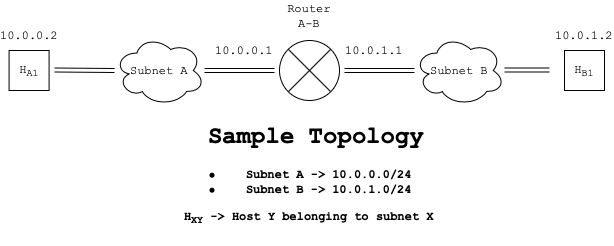
\includegraphics[width=\linewidth]{sample_topology.png}
        \caption{The sample topology we will set up throughout chapter \ref{chap:3}.}
        \label{fig:sample-topology}
    \end{figure}

    \section{Automating the Sample Topology}
        Listing \ref{lst:sample-topology} contains the shell script automating the deployment of the network showcased on figure \ref{fig:sample-topology}. The script itself contains messages that are to be printed to the user which clarify its operation to a great extent.\\

        \subsection{Running the Script}
            As seen on \texttt{line 1} of listing \ref{lst:sample-topology} this script is to be tun within a \texttt{bash} shell. This can be accomplished in one of two ways as shown on \ref{lst:bash-script}. As we will later look into, the script is to be run by \texttt{root} so that it can carry out the needed operations. This amounts to prepending the command we choose to run the script by \texttt{sudo}.\\

            \begin{lstlisting}[language = bash, caption = Running a \texttt{bash} script., label = lst:bash-script]
                # Making the script executable and running it.
                chmod +x <script-name> && sudo ./<script-name>

                # Spawning a privileged shell and running the script in it.
                sudo bash <script-name>
            \end{lstlisting}

        \subsection{Checking the Script is Run by \texttt{root}}
            The privileged user in \texttt{UNIX}-based systems is identified by a \texttt{UID} (\texttt{U}ser \texttt{ID}) of \texttt{0}. When a program is run, the associated process will have the \texttt{UID} of the user who launched it. Some program's permissions allow it to run with a different \texttt{UID} than that of the user executing it: this is wha we call the \texttt{EUID} (\texttt{E}ffective \texttt{UID})). In any case, if the \texttt{EUID} of a process evaluates to \texttt{0} it is being run by \texttt{root}. This is what is being checked by \texttt{lines 3-7} on listing \ref{lst:sample-topology}. If the user running the script is not \texttt{root} we will simply abort execution whilst warning the user.\\

        \subsection{Automatically Tearing Down the Topology}
            As seen in \texttt{lines 9-17}, the script shown on listing \ref{lst:sample-topology} is prepared to dismantle the network topology it brings up when invoked a second time. The trigger for this behaviour is passing a parameter when running the script. Any parameter will cause the removal of the entire virtual network: this is not the best practice when writing code but it simplifies handling the arguments passed to the script. We are concerned with clearly portraying the technologies discussed in chapter \ref{chap:2}, not with teaching the user how to write proper shell scripts. In any case, running \texttt{sudo bash <script-name> quit} will dismantle the sample virtual topology.\\

        \lstinputlisting[language = bash, caption = Automatic deployment of the \textit{Sample Topology}., label = lst:sample-topology]{Code_snippets/sample_topology.sh}

    \section{Testing the Topology Is Working}
        Once the script shown on listing \ref{lst:sample-topology} has been run we should have a full-fledged virtual network at our disposal. The simplest way to check we do have full connectivity is checking one of the hosts can ``see the other''. we can accomplish our objective by running a shell within one of the hosts and then trying to \texttt{ping} the other. We can extract the appropriate \texttt{IP} addresses from figure \ref{fig:sample-topology}. Listing \ref{lst:sample-topology-test} shows how we can open up a shell within host $H_{A_1}$ and launch \texttt{ping} against host $H_{B_1}$.\\

        \begin{lstlisting}[language = bash, caption = Testing the Sample Topology., label = lst:sample-topology-test]
            # Spawn a shell within H-A-1
            docker exec -it h-a-1 bash

            # Ping H-B-1 3 times from H-A-1
            root@h-a-1:/$ ping -c 3 10.0.1.2

            # It should produce an output similar to:
                # PING 10.0.1.2 (10.0.1.2) 56(84) bytes of data.
                # 64 bytes from 10.0.1.2: icmp_seq=1 ttl=63 time=0.036 ms
                # 64 bytes from 10.0.1.2: icmp_seq=2 ttl=63 time=0.057 ms
                # 64 bytes from 10.0.1.2: icmp_seq=3 ttl=63 time=0.062 ms
                #
                # --- 10.0.1.2 ping statistics ---
                # 3 packets transmitted, 3 received, 0% packet loss,\
                    # time 2049ms
                # rtt min/avg/max/mdev = 0.036/0.051/0.062/0.011 ms

            # We can also run traceroute
            root@h-a-1:/$ traceroute 10.0.1.2

            # It should produce an output similar to:
                # traceroute to 10.0.1.2 (10.0.1.2), 30 hops max, 60\
                    # byte packets
                # 1  10.0.0.1 (10.0.0.1)  0.029 ms  0.039 ms  0.007 ms
                # 2  10.0.1.2 (10.0.1.2)  0.018 ms  0.023 ms  0.041 ms
        \end{lstlisting}

    Now that we have shown how to ``manually'' set up a simple network we begin to discover the challenges that will surely arise as their complexity grows. What is more, we also need to add additional functionalities such as moving end nodes around the network in a way that does not mangle the network's operation. The next chapter is devoted to providing a high level overview of our tool's design and operation together with a comprehensive collection of the actions it can and cannot perform.
